\section{Transfer Learning}

In the experiments part of the paper was describe a practical use of the purpose of the project with transfer learning. 

The formal definition of transfer learning is: \textquotedblleft Given a source domain $\mathcal{D}_{S}$, a corresponding source task $\mathcal{T}_{S}$, as well a target domain $\mathcal{D}_{T}$ and a target task $\mathcal{T}_{T}$, the objective of transfer learning now is to enable us to learn the target conditional probability distribution $\mathcal{P(Y_{T}|X_{T})}$ in $\mathcal{D}_{T}$ with the information gained from $\mathcal{D}_{S}$ to $\mathcal{T}_{S}$ where $\mathcal{D}_{S} \neq {D}_{T}$ or $\mathcal{T}_{S} \neq {T}_{T}$ "

So, transfer learning is a machine learning technique where a model trained on one task is re-purposed on a second related task. In the paper, the second related task is classification object and we chose to keep it.

The neural network for this part is the same of the first part, but we add an additional dense layer at the end, as in the paper.

We use the CFN weights that we have found at the end of the training of the CFN to initialize the \texttt{conv} layers of the standard AlexNet network. The other layers have Gaussian noise as initial weights. Then, those the \texttt{conv} layers are frozen during the process of training. In this way, this process allows rapid progress and improved performance when modelling the second task. In fact, we have only $8,441,637$ parameters to be trained with only one instance of the AlexNet.

\begin{figure}[!ht]
    \centering
    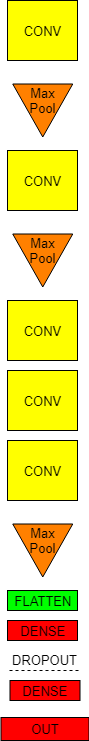
\includegraphics[scale=0.50]{images/FT_net.png}
    \caption{Architecture of the transfer learning neural network.}
    \label{fig:FT_net}
\end{figure}

The transfer learning experiment that is describe in the paper use a dataset named \textquotedblleft PASCAL VOC 2007". This dataset has 20 classes and $9,963$ images. We chose to use a different dataset to compare the results at the end of the training.

We select a dataset named \textquotedblleft Food 101" \cite{food_images} that have 100 classes and 1000 of images for each class. We choose to use a \textit{.h5} file for it but to read the images from files. We provide to build a list of relative path to every image of the dataset with the corresponding associate class. Every class is traduce to an integer number. 

The dataset was divided into 70\% training, 25\% validation and 5\% test.
We edit the images of the dataset in this way:

\begin{itemize}
    \item central squared crop of every image;
    \item resize at $225 \times 225$ pixel.
\end{itemize}

% We aren't able to have some results for this part.

% Now we present a comparison between the results of those two databases:

% TODO: Tabella di confronto tra risultati Pascal e Food


